\documentclass[12 pt]{article}
\usepackage{fancyhdr}
\usepackage[margin = 1 in]{geometry}
\usepackage{amsmath}
\usepackage{enumerate}
% \usepackage{indentfirst}
\pagestyle{fancy}
\usepackage{graphicx}
\usepackage[version=3]{mhchem}
\fancyhf{}
\usepackage{sectsty}	
\lhead{Andrew Wang}
\chead{CS/CNS/EE 155 Machine Learning \& Data Mining}
\rhead{Yue}
\sectionfont{\fontsize{15}{18}\selectfont}
\usepackage{graphicx}
\usepackage{array}
\newcolumntype{P}[1]{>{\centering\arraybackslash}p{#1}}
\newcolumntype{M}[1]{>{\centering\arraybackslash}m{#1}}
\usepackage[font=small,labelfont=bf]{caption}
\usepackage{float}

\begin{document}
	\begin{center}
		\section*{Homework 1}
	\end{center}
	
	
	\subsection*{1 Basics}	
	\textbf{Question A:} The hypothesis set is the set from which hypothesis, or approximations of the target function, is taken from. \\
	
	\noindent\textbf{Question B:} The hypothesis class of the linear model is of the form: w$^T$x + b. \\
	
	\noindent\textbf{Question C:} Overfitting occurs when the test error $>$$>$ training error, often implied by high variance. This can typically be attributed to the particular model learning specifics and noise of the training data too well to the extent that its performance is negatively impacted on testing data. \\
	
	\noindent\textbf{Question D:} Attaining more training data reduces variance which could alleviate the problem of overfitting. We could also use a validation set or k-fold cross validation so we have a means of evaluating specific models and thereby getting a measure for which models yield lower errors on the validation sets/ partition. \\
	
	\noindent\textbf{Question E:} The training set is the set we use to learn, i.e. fit parameters of the model. The testing set is the set we use to evaluate the performance of our full-trained model. We should not tune our model any further based on the testing set because doing so puts us at risk for having a final model that fits/ is biased towards the test set which would affect performance. \\
	
	\noindent\textbf{Question F:} One assumption is that the data is sampled independently of the "true" distribution. In addition, the outputs of the sampled data must be sufficiently diverse in that for the example of detecting spam, we need emails that are categorized as spam AND as not spam. If we only have emails that are spam, then learning would be rather pointless. \\
	
	\noindent\textbf{Question G:} X could consist of the emails in some parameterized vector form. For example, in class, we went over how we could break down each email into a vector based on the "bag of words" representation. Additional parameters such as length of email can also be taken in consideration. Y would just be [0, 1], a binary indicator of either the email is not spam or spam. \\
	
	\noindent\textbf{Question H:} K-fold cross validation involves partitioning the data into K equal-sized partitions. We train on $($K - 1$)$ partitions and evaluate on 1 partition. The cross validation procedure is then repeated K times with each of the K partitions used exactly once as the validation data. This ultimately allows for re-using of training data as test data.
 
	
	\subsection*{2 Bias- Variance Tradeoff}
	\noindent\textbf{Question A:}
	\[ E_S\big[ E_{out}(f_s)\big]\]
	\[ = E_S \Big[ E_x \Big[ (f_S(x) - y(x))^2 \Big]  \Big]\]
	\[ = E_x \Big[ E_S \Big[ (f_S(x) - y(x))^2 \Big]  \Big]\]
	\[ = E_x \Big[ E_S \Big[(f_S(x) - F(x) + F(x) - y(x))^2 \Big]\Big] \]
	\[ = E_x \Big[ E_S \Big[ (f_S(x) - F(x))^2 + (F(x) - y(x))^2 +
	2(f_S(x) - F(x))(F(x) - y(x)) \Big]\Big] \]
	\[ = E_x \Big[ E_S \Big[(f_S(x) - F(x))^2 \Big]\Big] + E_x\Big[ E_S \Big[ (F(x) - y(x)^2 \Big] \Big] + E_x \Big [ E_S \Big[ (2(f_S(x) - F(x))(F(x) - y(x)) \Big]\Big] \]
	\[ = E_x \Big[ E_s \Big [(f_S(x) - F(x))^2 \Big]\Big] + E_x\Big[(F(x) - y(x))^2\Big] + 0 \]
	\[ = E_x \Big[ E_s \Big[ (f_S(x) - F(x))^2 \Big]\Big] + E_x\Big[(F(x) - y(x))^2\Big] \]
	\[ = E_x \Big[ E_S \Big[ (f_S(x) - F(x))^2 \Big]\Big] + E_x\Big[(F(x) - y(x))^2 \Big]\]
	\[ = E_x\Big[Bias(x) + Var(x) \Big]\]
	\\
	
	\noindent\textbf{Question B:} \\
	\noindent
	\begin{figure}[h]
	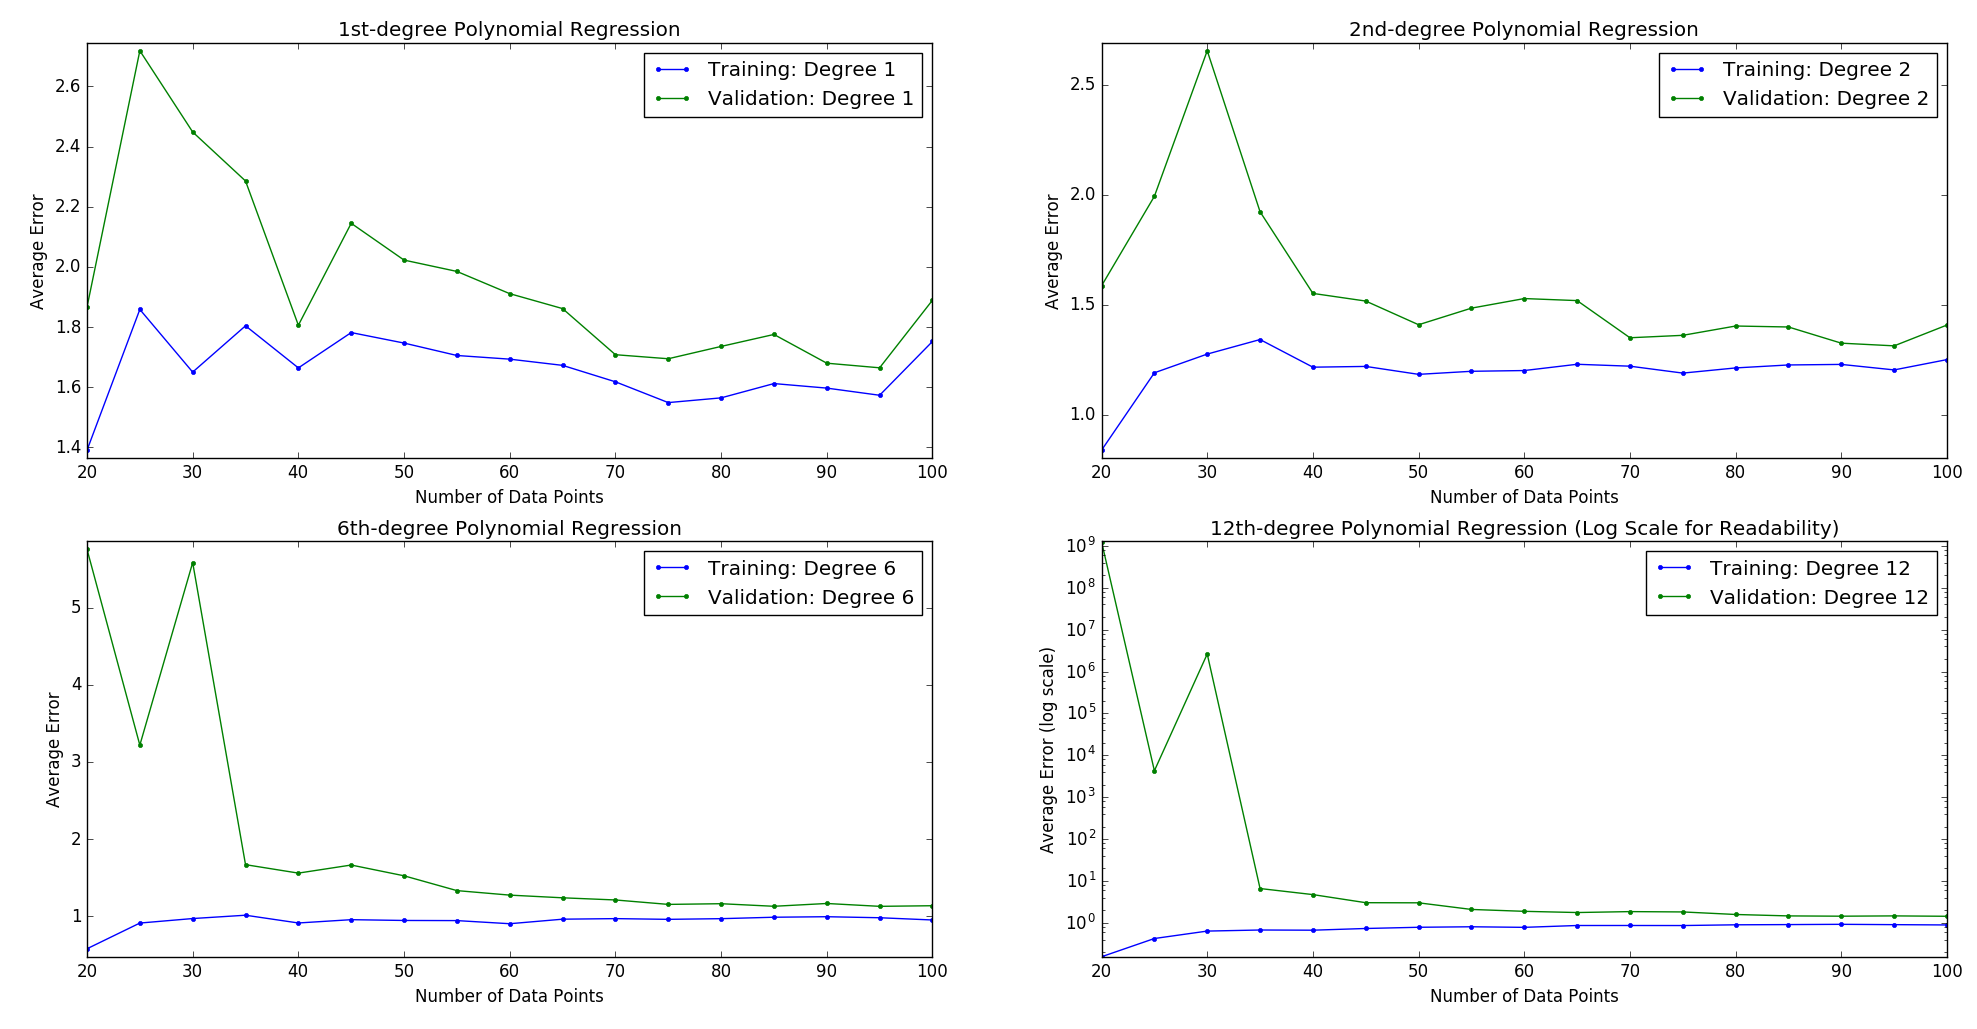
\includegraphics[width=17cm]{LearningCurves}
	\end{figure}	
	
	\noindent\textbf{Question C:} The 1st-degree polynomial regression has the highest bias. We can see that compared to the other models, the 1st-degree polynomial regression yielded highest average error for training data. Due to the low model complexity, the model is not able to fit the data well enough to capture the underlying trend. Additionally, we know that bias decreases with model complexity and because high bias implies underfitting, lower model complexities often imply high bias and thus underfitting.  \\
	
	\noindent\textbf{Question D:} The 12th-degree polynomial has the highest variance. We can see this from the very low training error, but enormous validation error at low $N$. This suggests that the model, with all its degrees, is fitting so much to subtleties (noise, random error, etc.) of the training data that it overlooks the true underlying relationship which is why the validation error is so high. In addition, variance increases with model complexity so it makes sense that the 12th degree polynomial yield high variance with implies overfitting.\\
	
	\noindent\textbf{Question E:} It appears that for the quadratic model, training error seems to plateau after 40 data points, although validation seems to decrease ever so slightly with larger $N$. This suggests that the quadratic model will generalize better with more data points. \\
	
	\noindent\textbf{Question F:} Intuitively, it makes sense that the training error is generally lower than validation error. We train on the training set, so the model directly uses the training data and is optimized on the training data. However, validation data is not used for training so the model does not use validation data for optimization. Because training data is used, the selected model tunes itself to fit the training data as opposed to validation data which the model does not see. Thus, the training error is generally lower than validation error. \\
	
	\noindent\textbf{Question G:} The 6th-degree polynomial regression would probably perform best on unseen data drawn from same distribution as the training data. Although the quadratic model appears to have lower validation errors for small $N$, we see that when we have more than 35 points, the 6th degree model has the lowest validation error which means it generalizes the best. 
	
	\subsection*{3 The Perceptron}
	\noindent\textbf{Question A:}
	\begin{center}
		\begin{tabular}{ |c|c|c|c|c|c|c| } 
			\hline
			t & b & w$_1$ & w$_2$  & x$_1$ &  x$_2$ & y \\ 
			\hline
			0 & 0 & 0 & 1 & 1 & -2 & 1\\ 
			1 & 1 & 1 & -1 & 0 & 3 & 1\\
			2 & 2 & 1 & 2 & 1 & -2 & 1\\
			3 & 3 & 2 & 0 & & &  \\
			\hline
		\end{tabular}
	\end{center}
	\noindent The final \textbf{w} = [2,0], b = 3. \\
	
	\noindent\textbf{Question B:} For a 2D data set, the smallest dataset that is not linearly separable consists of 4 data points. We can easily see this with: \\
	\indent +\\
	- \space\space\space\space\space\space\space\space\space -\\
	\indent +\\
	There's no line that can separate the above example so that all objects on on side of line are + and the other side -. In general, for a N-dimensional set, there are N+2 points in the smallest dataset that is not linearly separable. \\
	
	\noindent\textbf{Question C:} If the dataset is not linearly separable, the Perceptron Learning Algorithm will never converge. Based on question A, we know that for the PLA to stop, there must be no misclassified points to pick from for the updating of the weight vector. However, in the case where the data is not linearly separable, there will always be at least one misclassified point and because of such, the weight vector will always be updated and thus never converge.
	
	
	
	\subsection*{4 Gradient Descent}
	\noindent\textbf{Question A:} We add a w$_0$ = b and add x$_0$ = 1. Now, we have \textbf{w} = (w$_0$, w$_1$, w$_2$, ..., w$_d$) and \textbf{x} = (1, x$_1$, x$_2$, ..., x$_d$).\\
	
	\noindent\textbf{Question B:} \\

	\begin{eqnarray*}
		\partial_w \sum_{i=1}^{N} {(y_i - \textbf{w}^Tx_i)}^2 \\
		= \sum_{i=1}^{N} -2(y_i - \textbf{w}^Tx_i) x_i\\
	\end{eqnarray*} 
	
	\noindent\textbf{Question C: }(-0.22706695, -5.93069916, 3.93029727 -11.68517859, 8.74923223) is the final weight vector. It took 766 epochs. \\
	
	\noindent\textbf{Question D:} 
		\begin{figure}[H]
			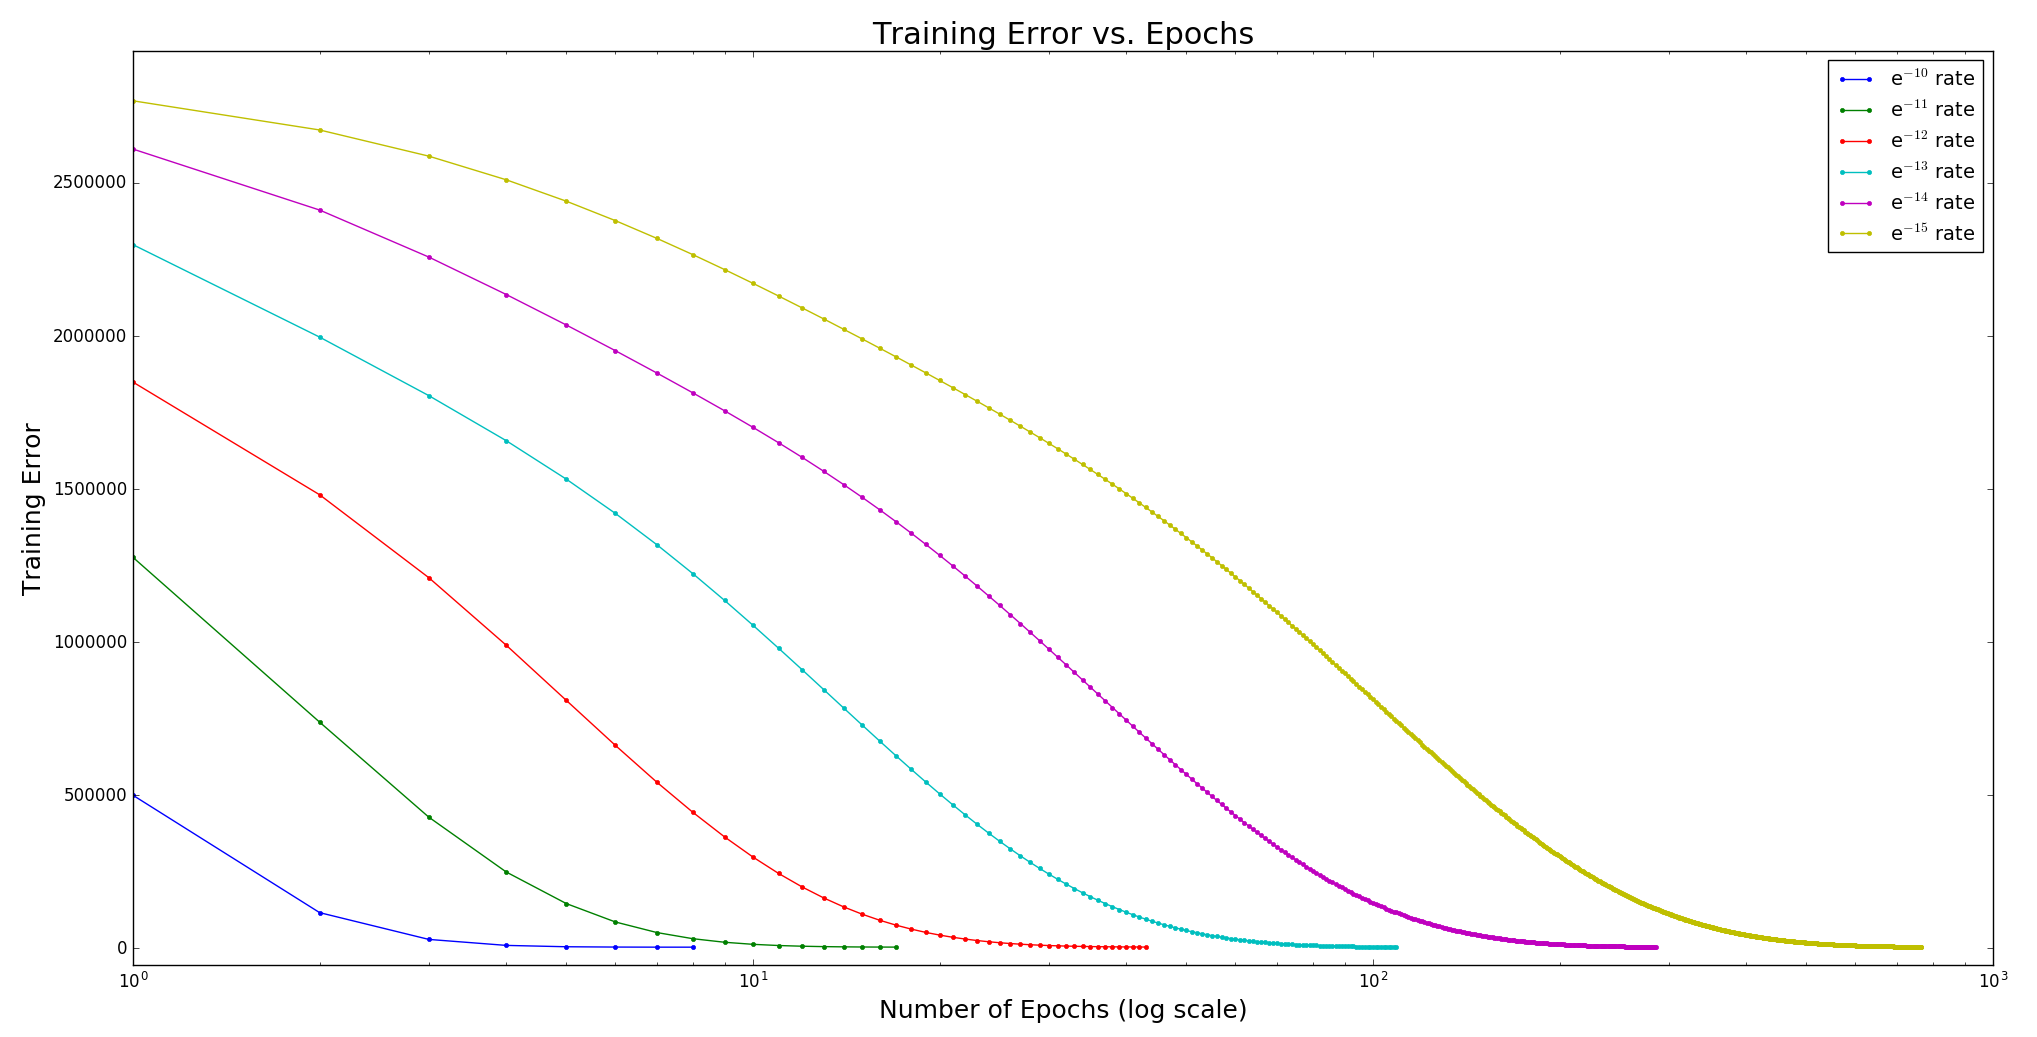
\includegraphics[width=17cm]{TrainingErrorEpochs}
		\end{figure} 
		
		\noindent We see that for a fixed learning rate, as the number of epochs increases, the training error goes down. This is as expected because the weights are adjusted with respect to the gradient, thereby minimizing the loss/ error. For a comparison between learning rates, we see that the smaller learning rates take more epochs to get the training error down. This makes sense as the change in weights is equal to the learning rate multiplied by the gradient. Thus, a bigger learning rate means a bigger change in weights which means less epochs to reach low training error. \\

	\noindent\textbf{Question E:} Using the closed form solution, I got the final weight vector \textbf{w} = (-0.31644251, -5.99157048, 4.01509955, -11.93325972, 8.99061096). This is very close to what we got from SGD of \textbf{w} = (-0.22706695, -5.93069916, 3.93029727 -11.68517859, 8.74923223). \\
	
	\noindent\textbf{Question F:} There can be situations where it may be impractical to use the closed form solution. For example, if your input matrix, \textbf{x}, is extremely large, taking the inverse of $\sum\limits_i\textbf{x}_i\textbf{x}_i^T$ for the closed form solution may be computationally intensive and time-consuming. No such operation is required for the SGD and thus, even as \textbf{x} increases in size, computational complexity does not significantly increase. \\
	
	\noindent\textbf{Question G:} In the convex case, we are guaranteed that all local optima are global optima. We do not have such case in the non-convex case. If the SGD is used on a non-convex learning problem, it is quite possible for it to converge to a local minimum, but not the global minimum. \\
	
\end{document}